\section{Introduction}
Differential equations are equations where the unknown is a function and the given equation gives us a relationship between the function and its derivative(s). Such equations are common in physics, economomics, etc. where we know how a quantity changes (i.e. its derivatives) but not necessarily how to determine the quantity at any given instant. Perhaps the most important differential equation is Newton's (second) law:
$$ ma = F $$
This equation tells us how force and acceleration, the second derivative of position, are interrelated. A similar example is that of the spring, where Hooke's law (in combination with Newton's law) tells us:
\begin{equation}\label{eqn:spring}
    m \cdot x''(t) = -k \cdot x(t)
\end{equation}

Without too much effort, we see that
$$ x(t) = \cos\left(\sqrt{\frac{k}{m}}t\right) $$
forms a solution to (\ref*{eqn:spring}), by which we mean that it satisfies the differential equation. Playing around a bit more we find that
\begin{equation}\label{eq:spring_soln}
    x(t) = A\cos\left(\sqrt{\frac{k}{m}}t\right) + B\sin\left(\sqrt{\frac{k}{m}}t\right)
\end{equation}
where $A$ and $B$ are some real numbers, all form solutions to (\ref*{eqn:spring}). As it turns out, this is what \textit{all} solutions to (\ref*{eqn:spring}) look like, although this is something we will prove later.

The parameters $A$ and $B$ are determined by the initial conditions that the differential equation needs to satisfy (in general 2 unknowns will require 2 initial conditions). Hence $A$ and $B$ in some sense parametrise the solution space. In such cases, we would like to have the parameters cover the entire solution space and for each set of parameters to correspond to a different solution.

\subsection{Solving Differential Equations}
There are two types of differential equations: ordinary differential equations, ODEs, (where the unknown function is in one variable) and partial differential equations, PDEs, (where the unknown function is in several variables). Our goal is to understand the quantity that the unknown function measures. Of course the best way to understand this quantity is by finding the unknown function. For example, the solutions above (see \autoref{eq:spring_soln}) instantly tell us that $x$ has periodic behaviour, not something immediate from the differential equation itself.

This is why there is so much interest in solving differential equations. ODEs can sometimes be solved analytically (see the above example), PDEs, almost never. However, we can often analyse differential equations themselves in order to make qualitative statements about the functions (how it changes, its limiting behaviour, points of equilibrium, etc.) and still learn meaningful information about the quantity being measured.

But perhaps we go any further, we should probably define what ODEs are
\begin{definition}[Ordinary Differential Equation]
An ODE is an equation of the form
$$ F(t, x(t), \dots, x^{(k)}(t)) = 0 $$
where $x$ is a vector valued function on an open interval $I \subset \R$ which is $k-$times continuous differentiable\footnote{In principle we don't need continuity of the $k-$th derivative, only its existence. However this does make things a lot nicer}. This is known as the implicit form of the ODE.
\end{definition}
If the codomain of $F$ is $\R^m$ with $m > 1$, we get a system of equations. Sometimes we can express the $k-$th derivative as a function of the lower order derivatives which gets the standard or explicit form.

We should also probably define what it means to solve an ODE.
\begin{definition}
A (classical) solution of an ODE $F(t, x(t), \dots, x^{(k)})(t) = 0$ is a function of class $C^k$ $\phi: I \to \R^n$, where $I \subset \R$ is an open interval, such that $F(t, \phi(t), \dots, \phi^{(k)}(t)) = 0$ for all $t \in I$.
\end{definition}
Note that not all ODEs can be solved. Consider, for example,
$$ \bigg|\frac{dy}{dx}\bigg| + |y| + 1 = 0 $$
Now, consider the following non-example. Suppose we are given the ODE
\begin{equation*}
    x + y \cdot y' = 0
\end{equation*}
We can define $y(x) = \sqrt{-(1 + x^2)}$ and we see that 
$$ y'(x) = \frac{-x}{\sqrt{-(1 + x^2)}} $$
which means that $x + y \cdot y'$ is certainly equal to 0. However, $y$ is not defined in the reals!

\begin{definition}
The general solution of an ODE is a formula for all possible solutions.
\end{definition}
The solution for $x$ above, (\ref{eq:spring_soln}), is an example of a general solution. It is normally no easy task to find the general solution to a differential equation as one needs to prove that they have indeed found \textit{all} possible solutions.

\subsection{Standard Trick}
There is a standard trick to turn a higher order ODE into a system of first-order ODEs which is a bit simple-minded but occassionally useful.
\begin{example}
Suppose we now have the equation
$$ mx'' = -kx - cx' $$
(one may think of this as introducing drag into our spring example). We can introduce new variables
$$ x_1 = x, x_2 = x' $$
allowing us to write
\begin{align*}
    \matrix{x_1\\x_2}' = \matrix{x_2\\ -\frac{-k}{m}x_1 - \frac{c}{m}x_2}
\end{align*}
\end{example}
In the general case of $F(t, x, x', \dots, x^{(k)}) = 0$, we define
\begin{align*}
    x_1 &= x\\
    x_2 &= x_1'\\
    x_3 &= x_2'\\
    \vdots\\
    x_k &= x_{k - 1}'
\end{align*}
thus allowing us to write $F(t, x_1, x_2, \dots, x_k) = 0$.

\section{Simple Examples}
We list a few `classic' examples of ODEs here. 

The first example is perhaps the simplest one, one could think of
\begin{equation}
    x' = 0
\end{equation}
It is easy to see that this is (only) solved by $x(t) = c$ where $c$ is some real constant (and $t$ is any real number). Indeed the Fundamental Theorem of Calculus (and Mean Value Theorem) tell us that this is the general solution, thus we get a solution space of 1-dimension. This means that a single parameter dictates every possible solution, in this case that parameter is $c$.

The second example we look at is a slightly generalised version of this
\begin{equation}
    x' = f(t)
\end{equation}
Once again using the Fundamental Theorem of Calculus and the Mean Value Theorem, we find that the general solution is
$$ x(t) = x_0 + \int_{0}^{t} f(s) dx $$
where once again our space of solution is one-dimensional, governed in this case by the constant $x_0$.

The third example is one where things get interesting (and also an incredibly important example).
\begin{equation}\label{eq:eg3}
    x' = ax
\end{equation}
In fact this is a whole family of differential equations for every $a \in \R$. Some minor knowledge of calculus tells us that
$$ x(t) = ce^{at} $$
is a solution to this differential equation (once again $c$ can be any real constant). However it is not immediately obvious that this is the general solution to the differential equation. Let us show that this is is the case.

Let $\tilde{x}(t)$ be any solution to the equation. Our claim is that (\ref*{eq:eg3}) is a constant multiple of $e^{at}$. We show this by proving that the ratio of the two functions is always constant
\begin{align*}
    \frac{d}{dt}(\tilde{x}(t) e^{-at}) &= \tilde{x}(t)(-a e^{-at}) + \tilde{x}'(t)(e^{-at})\\
    &= -a \tilde{x}(t) e^{-at} + a \tilde{x}(t) e^{-at}\\
    &= 0
\end{align*}

This example indeed illustrates a general principle for solving ODEs: guess and check. This is to say that it is often easier to guess an answer to an ODE and then verify that this solution works than find one analytically. 

\section{Useful Pictures}
We've said many times that solving ODEs is a difficult, often impossible, task. We reiterate that here: solving ODEs is a difficult, often impossible, task. However, it is the case that the ODE can give us a lot of information about its solution(s) which we often summarise in various pictorial formats.

A differential equation gives us a way of computing the slope of the tangent to the function at any given point (this is, after all, what the derivative measures). 
\begin{figure}[h]
    \centering
    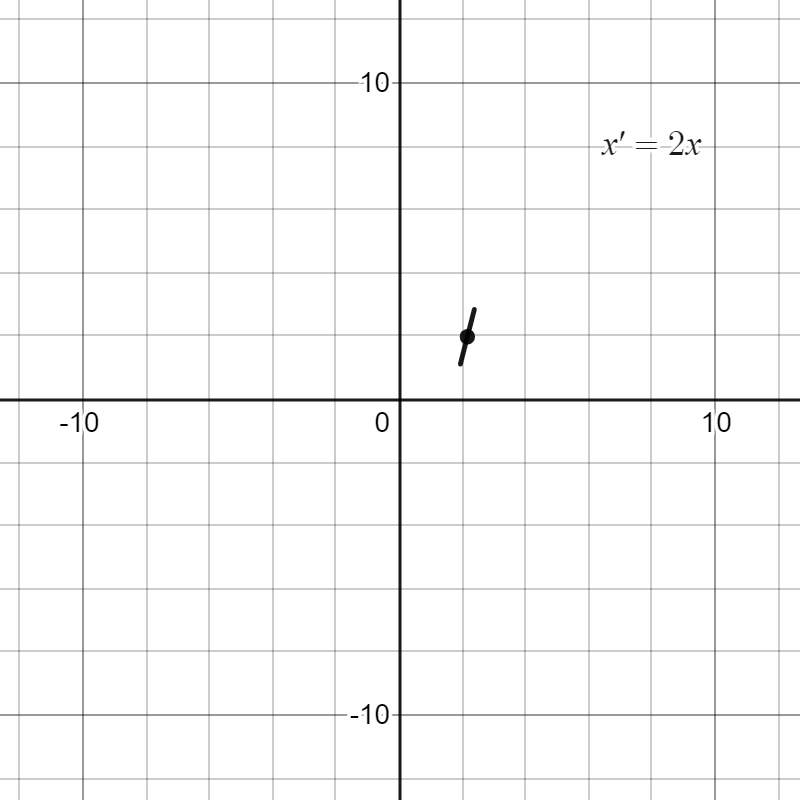
\includegraphics[scale=0.25]{Images/slope_field_1.png}
    \caption{Drawing the slope at one point}
    \label{fig:slope_one_pt}
\end{figure}

Thus one thing we can do to try and visualise the behaviour of the function is to find its derivative at every point \footnote{In practice, one often limits themselves to a finite set of points}. This called the slope field or direction field \footnote{Note the multiple names which will be a common theme here. It seems that the only thing harder than solving a differential equation is naming things related to them consistently.}
\begin{figure}[h]
    \centering
    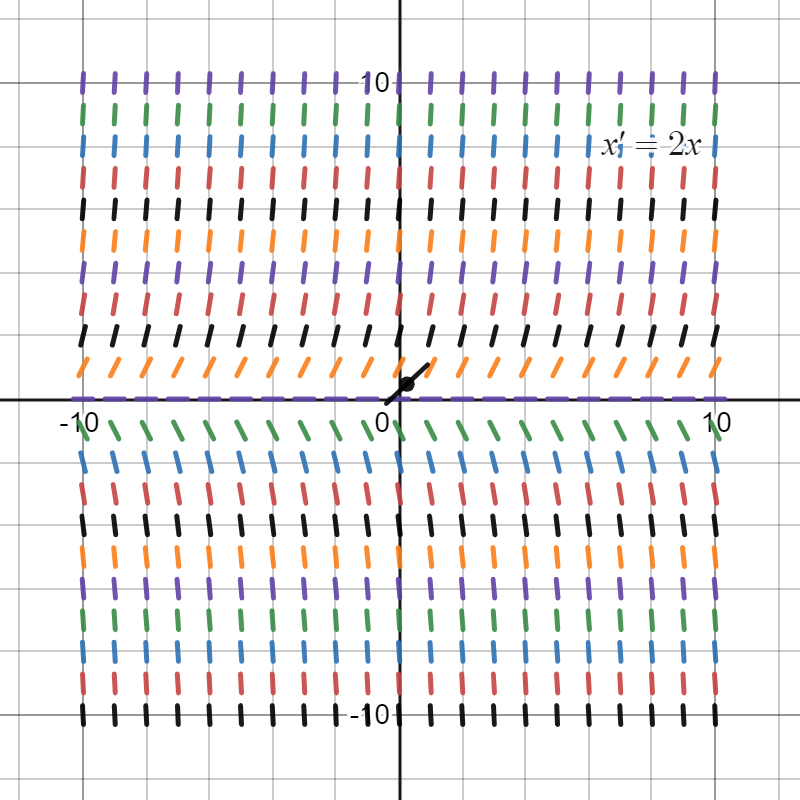
\includegraphics[scale=0.3]{Images/slope_field_2.png}
    \caption{Drawing a slope field on a grid for $x' = 2x$}
    \label{fig:slope_field}
\end{figure}

Seeing the slope field, we can turn the question of solving a differential equation to a visual one: we need to find a function which is tangent to every slope line. Of course there are a variety of possible solutions depending on where one starts from (one would hope that after deciding where to start from, there is only \textit{one} solution. we will see that in sufficiently nice conditions, this is the case). These solutions are also called integral curves. We illustrate a few examples below in \autoref{fig:slope_field_w_solns}. 

\begin{figure}
    \centering
    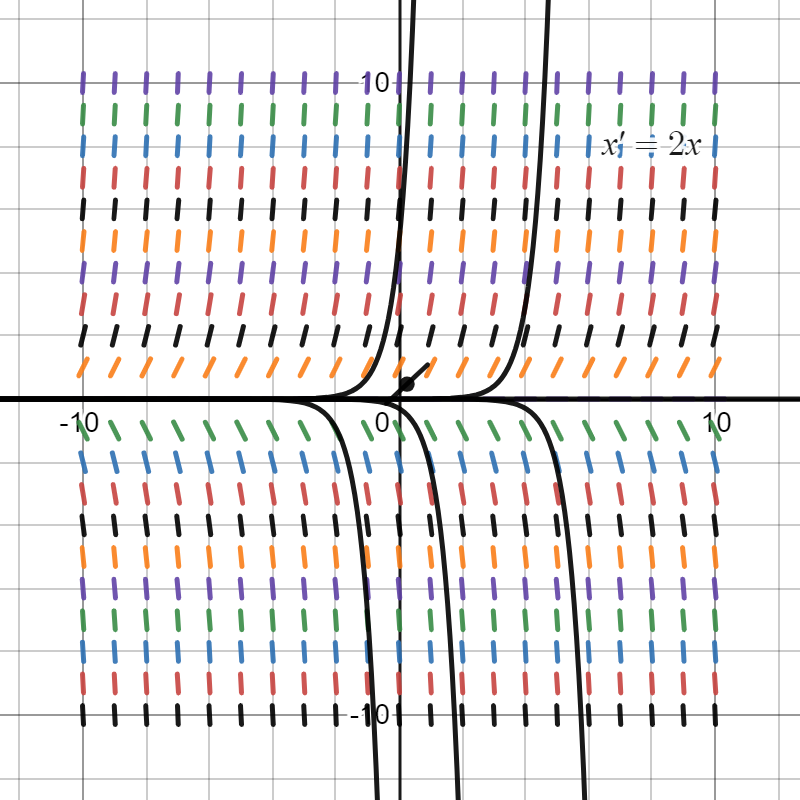
\includegraphics[scale=0.3]{Images/slope_field_with_solns.png}
    \caption{Slope field with some solutions (solutions illustrated in black)}
    \label{fig:slope_field_w_solns}
\end{figure}

We see that the slopes are all the same along any horizontal line. This is because the differential equation is independent of $t$. Such an ODE is called autonomous. For more general ODEs, we can still ask the question of what is set of points $(t, x)$ such that $f(t, x) = k$ for some constant $k$. In this case we call the set of points \textit{isoclines} (in particular then horizontal lines are isoclines for autonomous ODEs).\\

Consider the equation 
$$ x' = 2x $$
It is clear that the case with $x = 0$ (horizontal line in \autoref{fig:slope_field_w_solns}) is a special case as this is the only constant solution. In this case we call $0$ an equilibrium or steady state or stationary point. Consider what happens we are slightly above $x = 0$. In this case as $t$ goes to infinity (one often thinks of this time evolving), $x(t)$ gets further and further away from 0 (if this is modelling the position of a particle, then this shows that the particle grows further and further from its initial position (and at an increasing pace)). In particular if $x(t)$ is positive, it becomes more and more positive and if $x(t)$ is negative, it becomes more and more negative. We often represent this in what is called a phase line or phase portrait.

The fact that solutions near 0 move away from 0 as $t$ increases, means that although 0 is an equilibrium point, it is an unstable one (also called a source, if one imagines this as the flow a fluid). The opposite is of course a stable equilibrium (or sink) where solutions within some neighbourhood of the equilibrium point tend towards the equilibrium. Such a case occurs if we consider \autoref{eq:eg3} for $a < 0$. In this case 0 is again an equilibrium point, but now it is a stable one.

Notice the difference in behaviour between $a > 0$ and $a < 0$. Behaviour for all $a > 0$ is qualitatively the same and the same holds true for $a < 0$. In such cases we say that the equation $x' = ax$ for $a > 0$ (or $a < 0$) is stable (this is different from 0 being a stable point; in this case we are talking about the family of equations being a stable one.). 

It seems suggestive that we left out the case for $a = 0$ above. Indeed that is because the behaviour of the function is completely different for $a = 0$, since $x(t)$ is a constant in this case (this is exactly very example of an ODE we considered). It is at this point that 0 goes from being a source to a sink where the slightest change in $a$ causes it to go one way or the other. We say then that $a = 0$ is a \textit{bifurcation} in the 1-parameter family of equations $x' = ax$.

\begin{figure}[h]
    \centering
    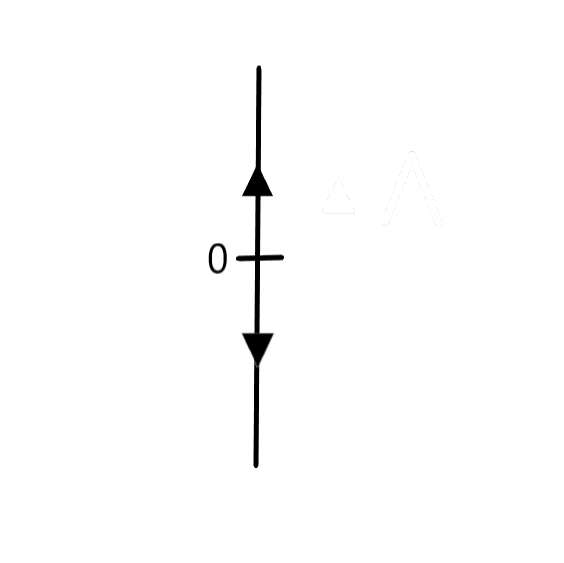
\includegraphics[scale=0.25]{Images/phase_line.png}
    \caption{Phase line/portrait for $x' = 2x$}
    \label{fig:phase_line}
\end{figure}

\section{The Logistic Equation}\label{sec:logistic-eqn}

Imagine you are trying to model the growth of a population. We know that if a population is small and is in ideal conditions (easily accessible food, few predators, lots of space, etc.). A population will grow exponentially. However, we also know that this cannot continue forever. As a population grows larger and larger, it will start pushing towards the limits of the available resources. In fact if the population grows too large for its environment (for example if there's not enough food or too many predators), then one would expect the population to decrease. A simple equation, known as the logistic equation\footnote{More precisely, the logistic equation is the solution to the differential equation with $N = 1$, but that's really more of a "tomato, tomato" situation}, that models this behaviour is 
\begin{equation}
    x' = ax \left( 1 - \frac{x}{N} \right)
\end{equation}
where $a \in \R$ is the growth rate of the population and $N$ is the carrying capcity or the ideal population size. Notice that if $x$ is small then $x' \approx ax$ and if $x > N$ (i.e. the population is greater than the carrying capacity) then $x' < 0$. We immediately see that this equation is still autonomous (we still have no $t$ in the equation) but it is no longer linear. This might already suggest that this is a somewhat more difficult problem than before (it is). Nevertheless, we can make our life a bit easier with one small assumption: without loss of generality we can take $N$ to be 1 (we just choose appropriate units of $x$ to make this work. One can think of $x$ modelling the proportion of the ideal population rather than the actual size of the population). We thus define
\begin{equation}
    f_a(x) = ax(1 - x)
\end{equation}

We see that $f_a(x)$ is 0 for $x = 0$ and $x = 1$ (these are hence our equilibrium points), positive if $x \in (0, 1)$ and negative otherwise. This already tells us that $x \equiv 0$ is an unstable solution while $x \equiv 1$ is a stable one. We can solve for other solutions to this differential equation (for other initial conditions) using a technique known as separation of variables.

We solve the ODE using separation of variables (see \autoref{sec:sep-of-var}).
\begin{align*}
    x' &= ax(1 - x)\\
    \frac{x'}{ax(1 - x)} &= 1\\
    \frac{1}{a} \int \frac{1}{x(1 - x)} dx &= \int 1 dt\\
    \frac{1}{a} \int \frac{1}{x} + \frac{1}{1 - x} dx &= t + c\\
    \frac{1}{a} \ln\bigg| \frac{x}{1- x} \bigg| &= t + c\\
    \bigg| \frac{x}{1- x} \bigg| &= e^{at + ac}\\
    \frac{x}{1 - x} &= c_2 e^{at}\\
    x &= \frac{c_2 e^{at}}{1 + c_2 e^{at}}
\end{align*}
Thus our solution is
\begin{equation}\label{eq:logistic_eqn}
    x(t) = \frac{c_2 e^{at}}{1 + c_2 e^{at}}
\end{equation}

\subsection{Parameterising the general solution}

Recall that that we also had special solutions to the equation, namely $x \equiv 1$ and $x \equiv 0$. We then see that $c_2 = 0$ recovers one of the solutions! Unfortunately the same is not true for the other solution (we would require $c_2 = \infty$). We can divide the numerator and denominator by $c_2$ to recover $x \equiv 1$ but we now lose $x \equiv 0$. This suggests that there might be a better parameterisation of the solutions. We see that 
$$ x_0 := x(0) = \frac{c_2}{1 + c_2} $$
We can solve for $c_2$ and substitute that into \autoref{eq:logistic_eqn} to get
\begin{equation}\label{eq:logistic_eqn2}
    x(t) = \frac{x_0 e^{at}}{1 - x_0 + x_0 e^{at}} = \frac{x_0}{(1 - x_0)e^{-at} + x_0}
\end{equation}
With this parametrisation, $x_0 = 0$ and $x_0 = 1$ get us the two special solutions.

Let's analyse this equation to see what we can learn of it. We will consider the case $a > 0$ since it is clear from the differential equation that cases for $a < 0$ are simply going to be reflections of the positive case (besides it is remarkably rare for populations to have a negative growth rate). Suppose the initial point $x_0$ is between 0 and 1. In this case, $x'$ is positive so $x$ will increase as $t$ increases (as we already predicted) and $x'$ will tend toward 0. However, looking at \autoref{eq:logistic_eqn2} we can see that no value of $t$ will make $x(t) = 1$. Hence $x = 1$ forms an asymptote. Suppose $x_0$ is greater than 1. Then $x'$ is negative. In this case, as before, $x$ will continually decrease, approaching $x = 1$ but never intersecting it. The most interesting case is when $x_0 < 0$. In this case, we know that $x(0) = x_0 < 0$. Note that at $t = 0$ the denominator starts of as a positive number, 1. However as $t$ grows larger and larger, $(1 - x_0) e^{at}$ will tend towards 0. Since $x_0$ is a fixed negative number, this means the denominator will be 0 at some point in time. In fact, we can work quite easily that this occurs at $t = \frac{1}{a}\ln(\frac{-x_0}{1 - x_0})$. This means that in this case the function will blow up to $-\infty$ in finite time.\footnote{We let the reader decide how they feel about negative population sizes exploding to $-\infty$.}

\begin{figure}[h]
    \centering
    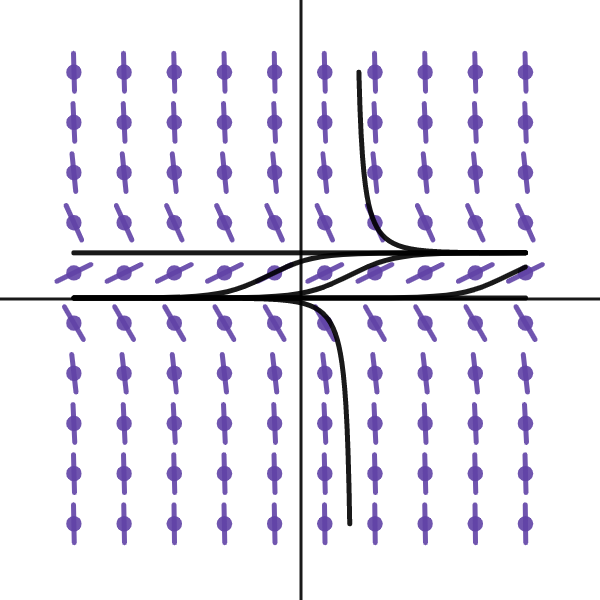
\includegraphics[scale=0.4]{Images/logistic_eqn_soln.png}
    \caption{Solutions to the logistic equation (solutions in black)}
    \label{fig:logistic_eqn_solns}
\end{figure}

